\documentclass{article}
\usepackage{fullpage}
\usepackage{amsmath,amssymb,graphicx,hyperref}
\usepackage{float}

\title{Speeding Up Matrix Multiplication with Machine Learning}
\author{Manan Bhatia}
\date{\today}

\begin{document}

\maketitle

\section{Introduction}
The basic operation of matrix multiplication serves as required in various areas including machine learning and computer science together with computer graphics and scientific simulations. The standard approach to matrix multiplication enables execution at a cubic speed \( O(N^3) \) when the square matrices have dimensions N. The algorithm optimisation requires improvement for large-scale systems because matrix multiplications serve as vital components of neural networks and transformer architectures in deep learning applications.

More efficient algorithms, such as Strassen's algorithm, demonstrates that the potential faster algorithms are possible, including the Copper-Winograd algorithm. However, the research for continuous faster algorithms has only been done by manual process, constrained by human intuition and vast combinatorial nature of practical solutions.

Through research presented in \textit{“Discovering Faster Matrix Multiplication”} it is found out that reinforcement learning technique serves as a method to extend previous work through accelerated mathematical exploration of matrix multiplication. The reinforcement learning agent AlphaZero serves as a basis for AlphaTensor to determine optimal tensor decompositions in finite factor spaces by playing a single-player game. The automated approach detected both standard and new algorithms which proved better than traditional methods for smaller matrix dimensions.

The research expands previous work by studying matrix multiplication mathematics while implementing AlphaZero-inspired reinforcement learning models to evaluate their achieved performance.
\begin{figure}[H]
    \centering
    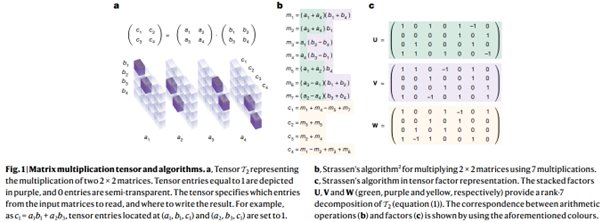
\includegraphics[width=0.6\linewidth]{Picture1.png}
    \caption{Tensor representation of matrix multiplication as a rank-3 tensor. Lower-rank decompositions reduce scalar multiplications. (Source: AlphaTensor paper)}
    \label{fig:tensor-representation}
\end{figure}

\section{Literature Review}
The search for enhanced matrix multiplication algorithms has proven challenging throughout many years in fields of mathematics and computer science. Research studies found ways to decrease the \( N^3 \) scalar multiplication requirement for matrix multiplication by exploiting mathematical structures in the algorithm.

The foundation for improving matrix multiplication processes came from classical methods. The time complexity reached approximately \( O(N^{2.81\ldots}) \) through Strassen's algorithm by converting two \( 2 \times 2 \) matrix multiplication into 7 recursive subproblems rather than 8. 
Coppersmith-Winograd algorithm developed this methodology to achieve matrix multiplication complexity at\(  O(N^{2.376}) \). The state-of-the-art matrix multiplication algorithms currently reach an \( O(N^{2.37}) \) complexity level but actual practical applications tend to use Strassen's method as an economical alternative for medium-scale matrices.

The process of understanding matrix multiplication uses tensor decomposition as an essential mathematical tool. The matrix multiplication operation can be understood as a rank-3 tensor but requires finding the most compact rank representation. The conversion to lower-rank expression requires fewer multiplication operations across scalars. The matrix multiplication tensor of size \( 2 \times 2 \times 2 \) finds its rank-7 decomposition through Strassen's algorithm. Through tensor decomposition researchers gain a unified perspective for both existing algorithm analysis and new algorithm discovery hence becoming an optimal method for optimisation research.

The application of reinforcement learning methods for mathematical discovery opens new possibilities in research. AlphaZero proved that software which links reinforcement learning to self-play with Monte Carlo Tree Search routing could reach superhuman levels in complicated games of Go and Chess. The article modified this framework to develop algorithm discovery along with AlphaTensor which is a reinforcement learning agent that understands tensor factorisation of matrix multiplication. The AlphaTensor system accomplished both the rediscovery of Strassen's algorithm and the identification of newly discovered algorithms that demonstrated better performance than traditional matrix multiplication methods when applied to small matrix sizes. 
The study demonstrated how RL stands as a forceful method for symbolically understanding matters and creating new algorithms.

The proposed synthesis of classical algorithms and tensor decomposition theory and reinforcement learning serves to expand scientific knowledge in matrix multiplication optimisation. The research will adapt AlphaTensor's reinforcement learning approach to evaluate discovered algorithms for their practical value in transformer computations which require heavy use of matrices.

\section{Methodology}
This project uses a defined procedure which includes the exploration and implementation and evaluation of machine learning algorithms to boost matrix multiplication speed. An approach with three main elements will lead the project which includes creating the mathematical foundation and designing the reinforcement learning system and evaluating the discovered algorithms. 

This project bases its foundation on comprehension of the mathematical concepts that govern matrix multiplication. The concept of tensor decomposition will be studied because it shows how matrix multiplication operates as a rank-3 tensor. Lower-rank decomposition of this tensor stands as the goal because it leads to fewer necessary scalar multiplications. The evaluation of new algorithms will use existing methods and tensor rank analysis and bilinear complexity comparison with Strassen's and Coppersmith-Winograd algorithms.

The present work adopts an AlphaZero framework to create a reinforcement learning system shaped after the approach from the article. In this setup the RL agent views matrix multiplication as a game that defines states through partial decomposition steps and employs actions through choices of matrix sub-block combination. MCTS explores while the neural network evaluates policies for the agent which improves its strategy through self-play during multiple iterations. The reward signals will be established through scalar multiplication counts to direct algorithm discovery toward less complex methods. A training process will operate on basic matrix dimensions \( 3 \times 3 \) to achieve successful algorithm discovery despite computational restrictions.

\begin{figure}[H]
    \centering
    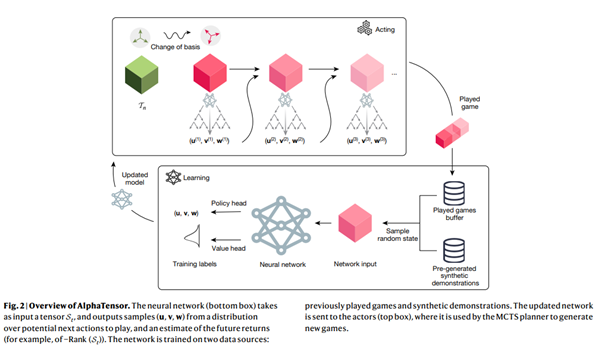
\includegraphics[width=0.6\linewidth]{Picture2.png}
    \caption{AlphaTensor's reinforcement learning framework for algorithm discovery. (Source: AlphaTensor paper)}
    \label{fig:alphatensor-framework}
\end{figure}

The research will analyse discovered algorithm performance through evaluations with traditional algorithms that include the classical cubic algorithm and Strassen's algorithm. The evaluation framework uses the count for scalar multiplication operations together with runtime performance measurements coupled with scaling abilities for bigger matrix sizes. A simplified transformer model will receive these discovered algorithms to determine their effect on the runtime of self-attention computations.

\begin{figure}[H]
    \centering
    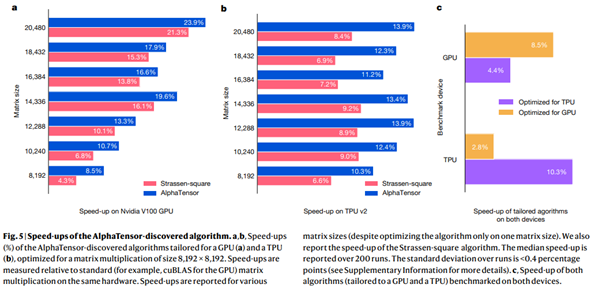
\includegraphics[width=0.6\linewidth]{Picture3.png}
    \caption{Speed ups of the AlphaTensor-discovered algorithm (Source: AlphaTensor paper)}
    \label{fig:speedups-alphatensor}
\end{figure}

The approach creates a systematic investigation of matrix multiplication algorithms through machine learning which extends human intuition capabilities beyond current boundaries.

\section{Contribution}
The research focuses on optimising matrix multiplication techniques to enhance their application in machine learning especially within reinforcing learning frameworks and transformer systems. The following aspects will be the focus of my work in implementation using both Python and Julia:

\subsection*{1. Exploring the mathematics of matrix multiplication and the significance of optimisation}
I will start the analysis by examining basic mathematical principles of traditional matrix multiplication algorithms followed by their computational difficulty evaluation. The research will examine fundamental algorithms starting from the straightforward \( O(N^3) \) approach alongside fastest methods that include Strassen's and Coppersmith-Winograd algorithms. The implemented algorithms through Python will enable performance evaluation and statistical analysis of their computational requirements. The analysis will include matrix optimisation approaches alongside the implementation of pruning and sparsity exploitation through Julia since it excels at running essential large numerical calculations.

\subsection*{2. Test reinforcement learning models inspired by the AlphaZero framework to discover novel matrix multiplication algorithms.}
I will use the AlphaZero framework to develop matrix multiplication algorithms through adapting its framework from its successful application to game-playing AI. The reinforcement learning environment will deploy Python together with OpenAI Gym or Stable Baselines3 platform to let agents choose matrix multiplication approaches while obtaining rewards from lower computation time and time complexity evaluation. Through this approach RL should discover improved matrix multiplication algorithms which will grow better with each subsequent iteration and learning cycle. When analysing time complexities of training algorithms during this task Julia will serve as the benchmarking tool.

\subsection*{3. Assess the performance of the algorithms identified by the model and explore potential improvements.}
The benchmark testing phase will assess the new algorithm variants through dual criteria of matrix multiplication speedups along with CPU/GPU time and memory consumption evaluations. The benchmark tests will be built using Python with NumPy and TensorFlow as popular data science libraries to operate on deep learning matrices. Due to its superior capabilities in high-performance numerical computations the Julia language will serve as the primary tool for extensive performance evaluations involving large matrix multiplications needed for neural network dataset training on MNIST and CIFAR-10. Analysis of the results will demonstrate which parts of the RL reward structure or performance tuning parameters need adjustment for peak performance enhancement.

\subsection*{4. Explore using matrix multiplication algorithms for self-attention in transformers.}
The study aims to determine how optimised matrix multiplication methods can be implemented for transformers especially inside their self-attention framework. I will modify the attention mechanism using Python and TensorFlow or PyTorch to integrate the optimised matrix multiplication algorithms that allow evaluation of performance effects on training duration and system memory consumption. The model inference times along with redundant calculation reduction in self-attention will be evaluated using Julia during heavy computation operations. The implementation of these modifications will prove the effectiveness of optimised matrix multiplication techniques for improving Transformer models during their training period and operational deployment.

I purpose to create an optimised line of matrix multiplication algorithms which will enhance computational efficiency and provide useful applications for machine learning particularly within reinforcement learning and transformer models. By using Python and Julia the project takes advantage of machine learning tools while gaining access to necessary computational power for processing large numerical data.

\section{Expected Results and Analysis}
The main objective of this work examines how reinforcement learning techniques might find superior matrix multiplication methods. The anticipated RL agent derived from AlphaZero capabilities will discover known matrix algorithms including Strassen's algorithm and potentially create new algorithms with minimised scalar multiplication counts.

At least three metrics will determine the performance evaluation of discovered algorithms compared against classical approaches including scalar multiplication counts as well as computational runtime duration and scalability capabilities. It is expected that the RL agent will achieve solutions at least equal to current algorithms when working with \( 2 \times 2 \) and \( 3 \times 3 \) matrix sizes. The optimisations show potential to decrease complexity when dealing with small to moderate matrix dimensions and may lead to extended scalability by implementing hierarchical decomposition approaches.

\begin{figure}[H]
    \centering
    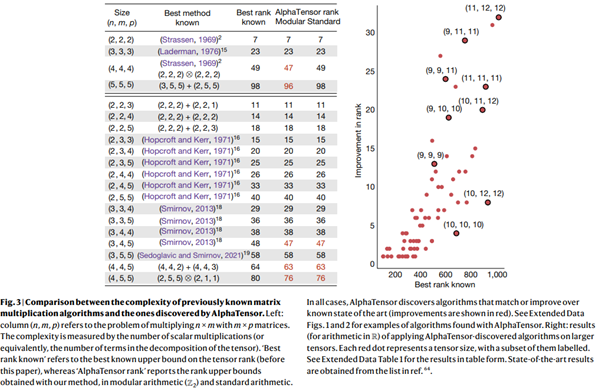
\includegraphics[width=0.6\linewidth]{Picture4.png}
    \caption{Comparison between the complexity of previous known matrix multiplication algorithms and the ones discovered by AlphaTensor. (Source: AlphaTensor paper)}
    \label{fig:comparison-alphatensor}
\end{figure}

A performance assessment of the discovered algorithms will conduct through their integration into basic transformer models for practical measurement of runtime efficiency. The researchers want to evaluate training time reductions for image classification on MNIST and CIFAR-10 datasets by implementing new algorithms instead of conventional matrix multiplication in their models.

Two main challenges exist regarding training RL agents for algorithm discovery which include high computational expense as well as stability issues for algorithms found specifically in larger matrix-based computations. The encountered obstacles offer research opportunities to develop combined strategies which unite learned algorithms with traditional methods for enhanced consistency and processing speed.

\begin{figure}[H]
    \centering
    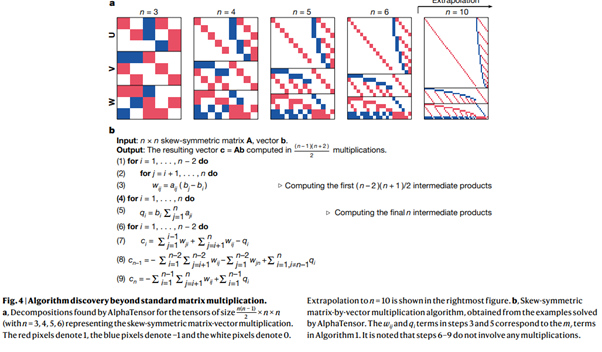
\includegraphics[width=0.6\linewidth]{Picture5.png}
    \caption{Algorithm discovery beyond standard matrix multiplication (Source: AlphaTensor paper)}
    \label{fig:standard-matrix}
\end{figure}

This study aims to demonstrate the practicality of deploying machine learning for algorithm discovery because it results in improved performance of matrix-based deep learning operations.

\section{Conclusion}
This work seeks to explore whether reinforcement learning techniques can find accelerated matrix multiplication algorithms based on AlphaZero framework success stories in discovering algorithms. The project starts with thorough investigation of matrix multiplication theoretical groundwork then creates a reinforcement learning system which approaches algorithm discovery as a gameplay format. Both theoretical and practical evaluations will assess the performance of discovered algorithms with special focus on their implementation in self-attention layers of transformers.

The successful execution of this project will yield new algorithms which minimise matrix product scalar multiplication requirements based on subsequent efficiency enhancements to speed-up machine learning model training. Smaller matrices will be the subject of first experiments, but the research aims to determine practical implementation potential of these discoveries for real-world systems.

The research direction includes improving both the RL training procedure and hardware optimisation strategies while expanding the solution approach towards additional linear algebra calculations. This paper wants to offer both insights about matrix multiplication along with new methods for using machine learning in basic algorithm investigation.

\section{References}
\begin{thebibliography}{9}
    \bibitem{fawzi} Fawzi, A., Balog, M., Huang, A. et al. Discovering faster matrix multiplication algorithms with reinforcement learning. Nature 610, 47-53 (2022). \url{https://doi.org/10.1038/s41586-022-05172-4}
    \bibitem{steassen} Strassen, V. Gaussian elimination is not optimal. Numer. Math. 13, 354-356 (1969). \url{https://doi.org/10.1007/BF02165411}
\end{thebibliography}

\end{document}